\documentclass[12pt]{article}
\usepackage[utf8]{inputenc}
\usepackage{amsmath,graphicx}
\usepackage[style=vancouver]{biblatex}
\addbibresource{references.bib}

\usepackage{fullpage}
\usepackage{lineno}
\usepackage{rotating}
\usepackage{xcolor}
\usepackage{subcaption}
\usepackage{graphicx}
\usepackage{longtable}
\usepackage{hhline}

\setlength{\parskip}{12pt}



\usepackage{newfloat}
\DeclareFloatingEnvironment[name={Supplementary Figure},fileext=lof]{suppfigure}



\setlength{\parindent}{0pt}
\setlength{\parskip}{6pt}



%%%%%% Title %%%%%%
\title{Structured inference...}

\author{}

%%%%%% Date %%%%%%
% Date is optional
\date{}


\begin{document}


\linenumbers

\maketitle

\begin{abstract}
Abstract

\end{abstract}

\clearpage


\section*{Introduction}
A citation \cite{lustig2023modelling}.


\section*{Methods}
\subsection*{Forward model}
Standard SEIR compartment model with a closed population of size $N$. Waning immunity is modelled via a transition through a sequence of two recovered (immune) compartments and from the second recovered compartment to the susceptible compartment. 
\begin{eqnarray}
\frac{dS}{dt} &=& -\lambda S + (2/t_R) R_2 \\
\frac{dE}{dt} &=& \lambda S - (1/t_E) E \\
\frac{dI}{dt} &=& (1/t_E) E - (1/t_I) I \\
\frac{dR_1}{dt} &=& (1/t_I) I - (2/t_R) R_1 \\
\frac{dR_2}{dt} &=& (2/t_R) (R_1-R_2) 
\end{eqnarray}
where $\lambda$ is the force of infection defined as
\begin{equation}
    \lambda(t) = \frac{R_0}{N} \left( \frac{I(t)}{t_I} + i(t)\right)
\end{equation}
Here $i(t)$ is a pre-specified function that seeds infections into an otherwise fully susceptible population. We define
\begin{equation}
    i(t) = i_0 \phi\left(\frac{t-t_s}{\sigma_s}\right)
\end{equation}
where $i_0$ is the number of seed infections, $t_s$ is the time of the maximal seeding, $\sigma_s$ is a parameter controlling the duration of the seeding event, and $\phi(.)$ is the standard normal probability density function. The model is initialised with $S(0)=N$ and all other variables equal to zero. Parameters as shown in Table 1.

We assume that, on average, a fixed proportion $p_\mathrm{obs}$ of infections are observed. This could represent surveillance data, for example the number of confirmed cases under the assumption that surveillance effort is steady over time. Alternatively it could represent a defined clinical outcome, such as hospital admission. There is an average lag of $t_\mathrm{obs}$ from the time an individual becomes infectious to the time they are observed. These assumptions are modelled via the differential equations
\begin{eqnarray}
    \frac{dC_1}{dt} &=& (p_\mathrm{obs}/t_E) E - (1/t_\mathrm{obs}) C1 \\
    \frac{dC_2}{dt} &=& (1/t_\mathrm{obs}) C_1
\end{eqnarray}
Here, $C_1$ represents the number of infected individuals who will be observed but have not yet been observed, and $C_2$ is the cumulative number of observed infections. The expected number of observations per day at time $t$ is denoted $Y_t$ and is equal to $(1/t_\mathrm{obs}) C_1$.

In addition, we assumed observations are subject to multiplicative Gaussian noise with fixed standard deviation $\sigma_\mathrm{obs}$. Hence, the observed data on day $t$ is
\[
\hat{Y_t} \sim N(Y_t, \sigma_\mathrm{obs}^2 Y_t^2)
\]
rounded to integer values. This is a crude noise model for count data - alternatives could include log-normally distributed observations with mean $Y_t$, negative binomially distributed observations with mean $Y_t$ or Poisson distributed observations with mean $N(Y_t, \sigma_\mathrm{obs}^2 Y_t^2)$.



\begin{table}
\begin{tabular}{ll}
\hline
Parameter & Value \\
\hline
Basic reproduction number  & $R_0=1.3$ \\
Latent period & $t_E=2$ days \\
Infectious period & $t_I=4$ days \\
Immune period & $t_R=300$ days \\
Proportion of infections that are observed & $p_\mathrm{obs}=0.01$ \\
Mean time from onset of infectiousness to being observed & $t_\mathrm{obs}=3$ days \\
Multiplicative noise s.d. & $\sigma_\mathrm{obs}=0.2$ \\
Number of seed infections & $i_0=20$ \\
Time of maximal seeding & $t_s=10$ days \\
Parameter controlling duration of seeding & $\sigma_s=1$ day \\
Population size & $N=5$ million \\
\hline
\end{tabular}
\end{table}

\subsection*{Structured inference}
A naive approach would be to do ABC rejection to infer the values of model parameters or some subset of them (note some parameters will be non-identifiable). This approach has the advantage of being conceptually simple and straightforward to implement. However, it is highly inefficient particularly if the number of parameters to be inferred is large, which is likely to be the case for models that capture more complexity of the epidemiological dynamics. A large number of runs of the forward model may incur a significant computational cost. 

Idea for structured inference: suppose we want to fit a selection of model parameters, say $R_0$, $t_I$, $t_R$ and $p_\mathrm{obs}$. Instead of doing naive ABC rejection in this 4 dimensional parameter space, consider the following method that samples parameter values from the 3-dimensional space $(R_0,t_I,t_R)$ and optimizes the fourth parameter $p_\mathrm{obs}$:
\begin{enumerate}
    \item Sample a parameter combination from the 3-dimensional space $(R_0,t_I,t_R)$.
    \item Run the forward model with the chosen values of $(R_0,t_I,t_R)$ and $p_\mathrm{obs}=1$.
    \item Note that, when other model parameters are fixed, the mean observations $C_t$ are directly proportional to $p_\mathrm{obs}$. Therefore, the optimal value of $p_\mathrm{obs}=p_\mathrm{obs}^*$ (i.e. the value that minimises the distance function or likelihood function with respect to the data) can be trivially found without rerunning the forward model. 
    \item Record this value of the distance function against the parameter combination $(R_0,t_I,t_R,p_\mathrm{obs}^*)$ and repeat to obtain a sample of $(R_0,t_I,t_R,p_\mathrm{obs})$ values.
    \item Filter as per standard rejection approach or more sophisticated ABC algorithm such as ABCSMC.   
\end{enumerate}









\section*{Results}
An example run of the forward model is shown in Fig. \ref{fig:forward_model}.


\begin{figure}
    \centering
    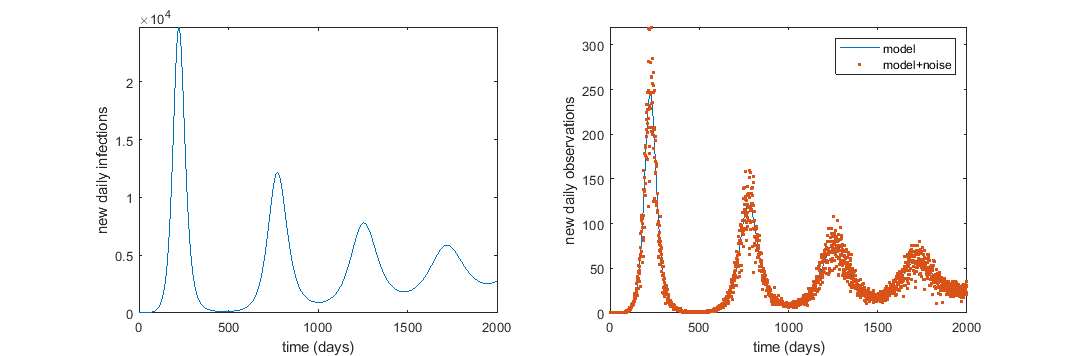
\includegraphics[width=\textwidth]{figures/forward_model.png}
    \caption{Example results from the forward model showing: (a) new daily infections and (b) new daily observations (blue curve = mean; red dots = noisy observations). }
    \label{fig:forward_model}
\end{figure}







\section*{Discussion}

\subsection*{Acknowledgements}


\printbibliography




%%%%%%%%%%%%%%%%%%%%%%%%%%%%%%%%%%%%%%%%%%%%%%%%%%%%%%%%%%%%%%%%%%%%%%%%%%%%%
% Supplementary Materials

\clearpage
\setcounter{page}{1}
\setcounter{section}{0}
\setcounter{equation}{0}
\setcounter{figure}{0}
\setcounter{table}{0}
\renewcommand\thepage{S\arabic{page}}
\renewcommand\thesection{S\arabic{section}}
%\renewcommand\thesubsection{S\thesection.\arabic{subsection}}
\renewcommand\theequation{S\arabic{equation}}
\renewcommand\thefigure{S\arabic{figure}}
\renewcommand\thetable{S\arabic{table}}

\begin{center}
    {\Large\bf Supplementary Material}
\end{center}

\tableofcontents 

\clearpage



\begin{refsection}





\begin{suppfigure}
    \caption{Supplementary Figure}
    \label{fig:}
\end{suppfigure}



\clearpage

\printbibliography[heading=subbibliography]
\end{refsection}



\end{document}

